% !TEX endcoding = UTF-8 Unicode
% !TEX TS-program = pdflatex
% !TEX spellcheck = en_US

\documentclass[a4paper, 12pt, oneside]{book}
\usepackage[T1]{fontenc}
\usepackage[utf8]{inputenc}
\usepackage[ italian, english]{babel}% la priorità è data all'ultima lingua
\usepackage{verbatim}
\usepackage{geometry}
\geometry{a4paper, top=4cm, bottom=2.5cm, left=3cm, right=3cm, heightrounded, bindingoffset=0mm}
\usepackage{graphicx}
\usepackage{caption}
\captionsetup{tableposition=top, figureposition=bottom, font=small}
\captionsetup{format=hang, labelfont={sf, bf}}
\usepackage{fancyhdr}
\usepackage{booktabs}
\usepackage{mathtools}
\DeclarePairedDelimiter{\abs}{\lvert}{\rvert}
\usepackage{subfig}
\usepackage{amsfonts}
\usepackage{bbold}
\usepackage{braket}
\usepackage{amsmath,bm}
\usepackage{amssymb}
\usepackage{microtype}
\usepackage{bigstrut}
\usepackage{mathrsfs}
\usepackage{multirow}
\usepackage{wasysym}
\usepackage{feynmf}
\usepackage{epstopdf}
\usepackage{rotating}
\usepackage{hyperref}
\usepackage{helvet}
\usepackage{multirow}
\RequirePackage{xspace}
\usepackage{xcolor}
\usepackage{afterpage}
\usepackage{pdfpages}
\usepackage{gensymb}

\begin{document}

\includepdf{frontespizio.pdf} %aggiunge frontespizio
\setcounter{page}{1}
\pagenumbering{roman}
\tableofcontents %%indice


\chapter*{Introduction}
\setcounter{page}{1}
\pagenumbering{arabic}

\addcontentsline{toc}{chapter}{Introduction}
\label{ch:Introduction}
Naples is the city where I was born. It is in Italy and is a wonderful city, near the sea and with a mild climate.\\ 

In this city you can eat very good food everywhere, from pizza to pasta and thousand of different cakes.\\ 

It is a city of art, full of museums and churches where you can find different art styles as Baroque, Neoclassicism and Romantic.\\

It is historic since the city was conquered by different population in the past as Angevin and Aragonese.\\ 

The people are very kind with everyone and it is an alive city also for night life.\\

It is a city of culture, indeed, there are different universities which are very important as University Federico II that is one of the oldest in the world.\\

The site Teleport (\cite{Teleport}) asserts:
\begin{quote}
\textit{Naples, Italy, is characterized by reasonably priced housing. Our data reflects that this city has a good ranking in health-care and tolerance}.
\end{quote}
The site also considers Naples as 17th from a total of 163 countries for what each country on earth contributes to the common good of humanity, and what it takes away, relative to its size.\\

The mayor is trying to give an impulse to the city. He is facing the criminality and dealing with public debt, aiming to increment tourism. In the $2014$ and $2013$ he could get the charge to host respectively the \textbf{Copa Davis} and \textbf{Copa America}.\\

Naples is a city with a very high density of population so it could be a good investment for a local as a restaurant, or hotels, or pizza shop, coffee shop.\\

I want to use data to show what is the best area for an investment by stakeholders in these city.

\chapter*{Data Requirements}
\addcontentsline{toc}{chapter}{Data Requirements}
\label{ch:dataRequirements}
Naples is structured in Municipalities and Neighborhoods. There are 10 municipalities and 31 neighborhoods. I want to find the best area for an investment in commercial area. So I want to get the venues for every municipality, do a clustering of municipalities according their venues and then find the area. Mainly I need for this geospatial data. In particular, the data I will need for my notebook are:\\
\begin{itemize}
\item[-] Data for economy of the city. I will use BeautifulSoap\footnote{BeutifulSoap is a powerful Python library for scraping website} to scrape these data from Wikipedia \cite{economics};

\item[-] Data for municipality and neighborhoods. I will use BeautifulSoap to scrape these data from Wikipedia\cite{municipalities};

\item[-] Data for boundaris of every municipality. I will download the data from open data of the website of the city\cite{opendata}. These data are in the shapefile format. This format is a GIS (Geospatial Information System) standard for geospatial data. Every data is described in the standard WKT (Well Known Text) that describes an element of a map with Point, Linestring, Polygon. In this case the data are polygons that are difficult to manipulate. Yet, from polygons is possible to extract the boundaries as Linestring and the centroids as Point. I did this with an open-source tool QGIS. With shapefiles of boundaries and centroids it is easier to visualize Municipalities on Folium\footnote{Folium is a Python library to visualize geospatial data on a map} map. In figure \ref{fig:qgis_boundaries} you can see an example of what I mean.;

\item[-] Data for climate of the city. Being a city of sun, with a good climate, it is full of tourists the whole year. I will scrape them from a site\cite{climate} with BeautifulSoap;

\item[-] Data from Foursquare API\footnote{he Foursquare Places API provides location based experiences with diverse information about venues, users, photos, and check-ins } to extract venues for every municipality. The referring point for every municipality is the centroid of the municipality extracted as seen before;

\end{itemize}

\begin{figure}[!htb]
		\centering
		\scalebox{0.3}[0.5]{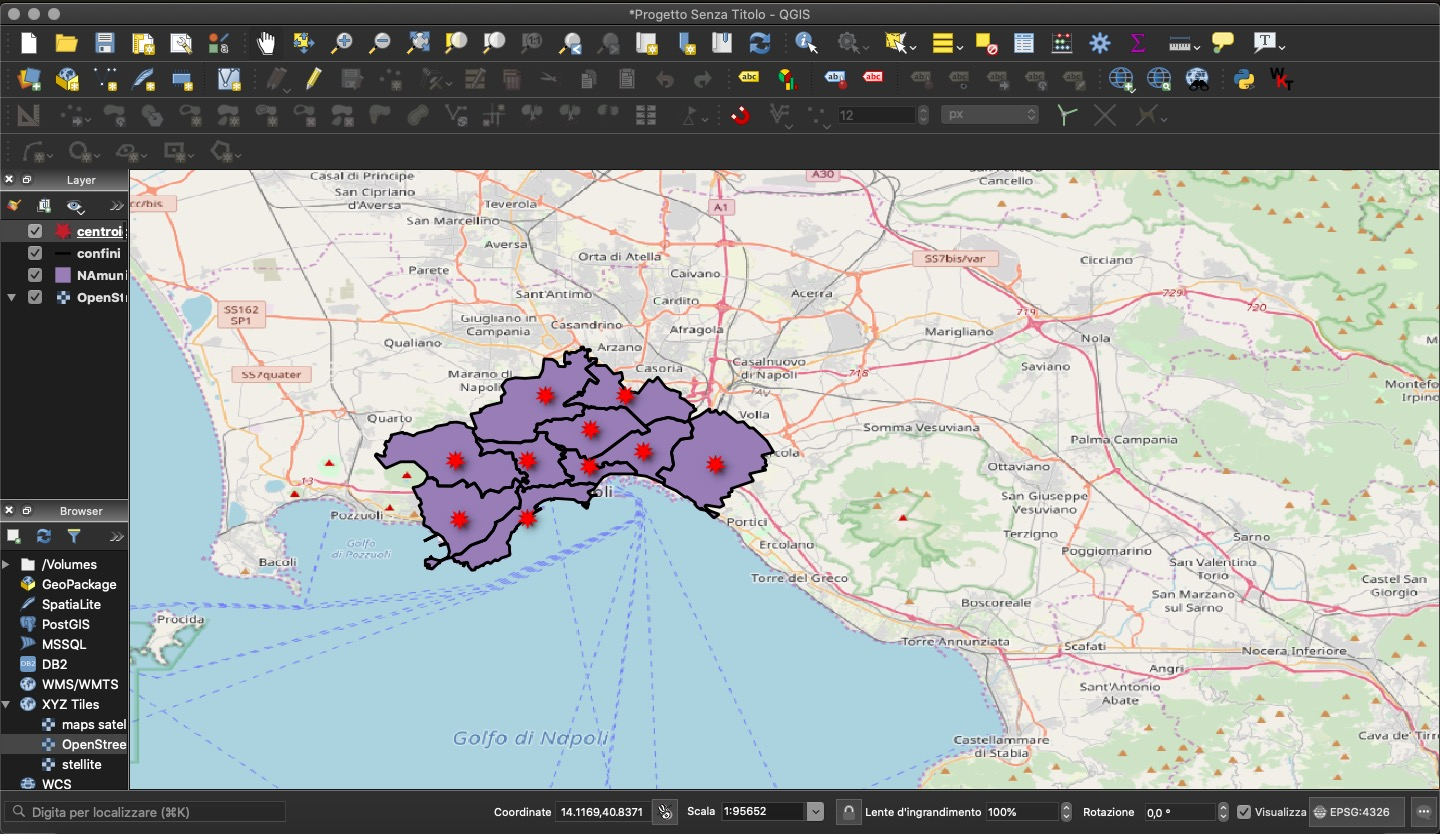
\includegraphics{immagini/qgis_boundaries.jpg}}
		\caption{Example of shapefile imported in QGIS. In violet the polygons representing the municipalities. In black the boundaries. In red star the centroids. }
		\label{fig:qgis_boundaries}
	\end{figure}



 As I mentioned the idea is to cluster municipality by venues, analyze the features of clusters. Then do a heat-map for the area of investment described previously and for every area find what is the best place to invest using density map or contour map.



\chapter*{Data collection and Understanding}
\addcontentsline{toc}{chapter}{Data Collection and Understanding}
\label{ch:dataCollection}
In this chapter we will see the collection of the data and the analysis of them. It's a fundamental step for preparing to modeling the problem. 

\section*{Analyze economy of the city} 
\label{sec:economy_city}
Naples is Italy's fourth-largest economy after Milan, Rome and Turin, and is the world's 103rd-largest urban economy by purchasing power, with an estimated 2011 GDP of US dollar 83.6 billion, equivalent to $\$$ 28749 per-capita. 

Naples is a major cargo terminal, and the port of Naples is one of the Mediterranean's largest and busiest. The city has experienced significant economic growth since World War II.

Naples is a major national and international tourist destination, being one of Italy and Europe's top tourist cities. Tourists began visiting Naples in the 18th century, during the Grand Tour. In terms of international arrivals, Naples was the 166th-most-visited city in the world in 2008, with 381000 visitors (a 1.6 per cent decrease from the previous year), coming after Lille, but overtaking York, Stuttgart, Belgrade and Dallas \cite{economics}.\\

Figure \ref{fig:df_economy} shows how is distributed the economy of the city. Investment in hotel is just $3.7~\%$, commerce $14~\%$ so it could be a good investment in this area since the city is not filled.

\begin{figure}[!htb]
		\centering
		\scalebox{0.45}[0.5]{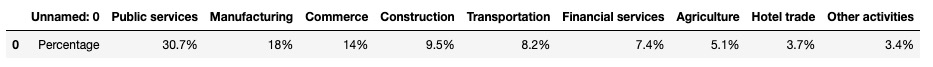
\includegraphics{immagini/dataframe_economics.jpg}}
		\caption{Dataframe describing economy of the city. }
		\label{fig:df_economy}
	\end{figure}


\section*{Build dataframe for Municipalities and Neighborhoods} 
\label{sec:df_municipality}
The dataset for municipalities and neighborhoods is scraped from Wikipedia\cite{municipalities} using the Python library BeautifulSoap and imported in the notebook as a Pandas dataframe\footnote{Pandas is a fundamental Python library for data analysis. A dataframe is data structure that can be imagined as a table with indices for rows and columns.}. In figure \ref{fig:df_mun_raw} you can see the raw data imported as a dataframe.
This dataset should be cleaned ad adjusted to be usable. Let's drop the columns "Presidente" indicatind the president for municipality (of no use in this case) and "Mappa" which contained the maps of each municipality in Wikipedia as images (clearly the images are not scraped). Then we should add a referring for latitude and longitude of every municipality. For that I download the open-data \cite{opendata} and I extracted the centroids of the polygons of municipalities to get the referring coordinates. As seen in the chapter "Data Requirements" I did it with the open source software QGIS and used the library shapefile of Python to read the centroids saved locally and then updated in my github\cite{dataset}.  

\begin{figure}[!htb]
		\centering
		\scalebox{0.45}[0.5]{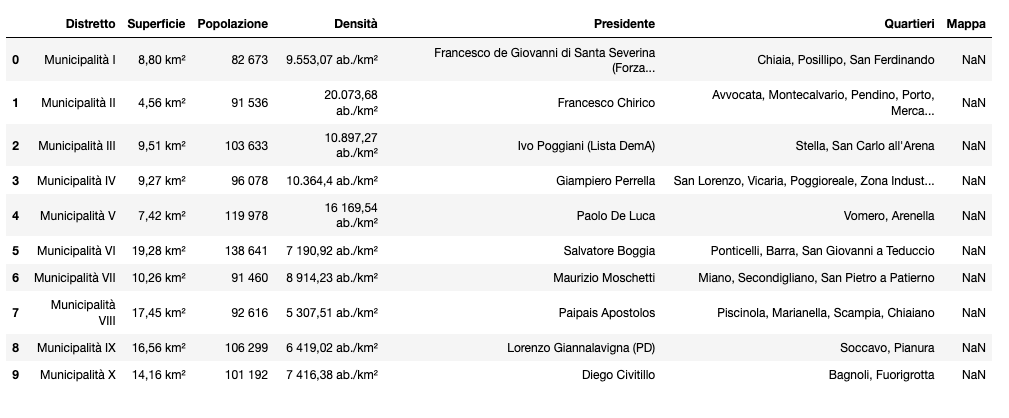
\includegraphics{immagini/df_mun_raw.png}}
		\caption{Dataframe describing raw data for municipalities and neighborhoods. }
		\label{fig:df_mun_raw}
	\end{figure}

After cleaned the dataframe and added latitude, longitude and number neighborhoods for every municipality, it appears as in figure \ref{fig:df_mun_cleaned}


\begin{figure}[!htb]
		\centering
		\scalebox{0.45}[0.5]{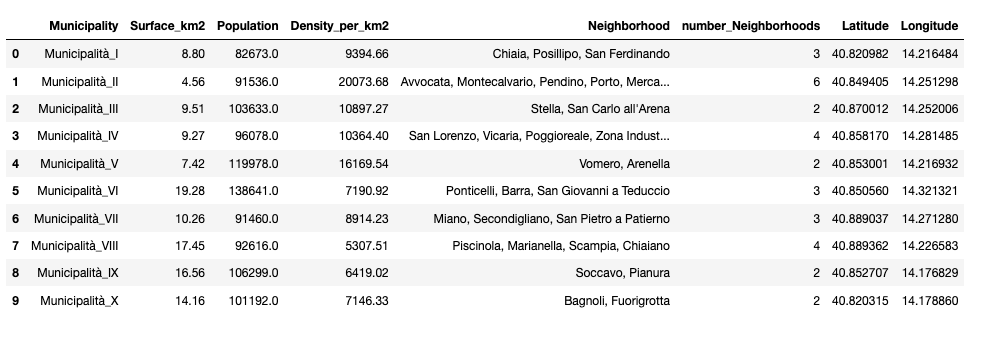
\includegraphics{immagini/df_mun_cleaned.png}}
		\caption{Dataframe describing cleaned data for municipalities and neighborhoods. }
		\label{fig:df_mun_cleaned}
	\end{figure}



Let's import also the boundaries in the same manner as centroids (the dataset is always in my github \cite{dataset}) and plot on the map the data for centroids and boundaries. See figure \ref{fig:map_municipality} showing a Folium map for boundaries and centroids.



\begin{figure}[!htb]
		\centering
		\scalebox{0.45}[0.5]{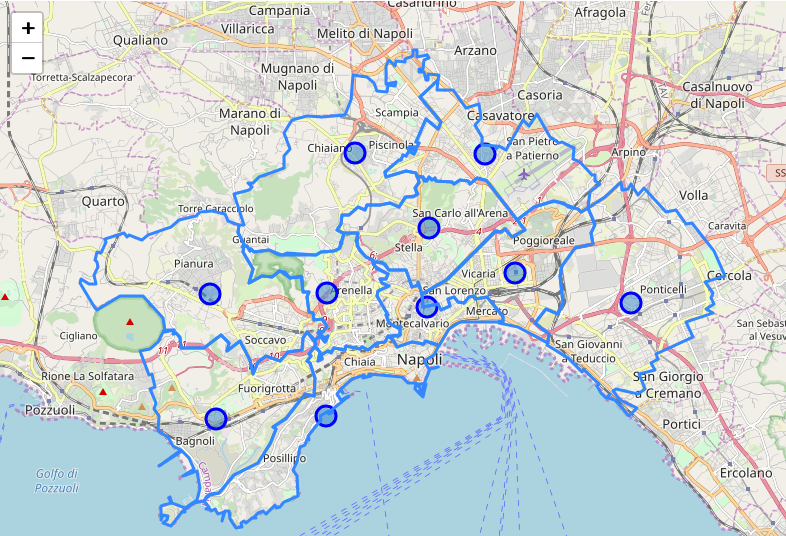
\includegraphics{immagini/map_municipality.png}}
		\caption{A Folium map for municipalities and neighborhoods. }
		\label{fig:map_municipality}
	\end{figure}


\section*{Extract climate data} 
\label{sec:climate}
As I mentioned previously, Naples is a city with a very mild climate. Let's see it. I scraped the data from a website \cite{climate} and in figure \ref{fig:df_climate} you can see a dataframe for climate data.



\begin{figure}[!htb]
		\centering
		\scalebox{0.45}[0.5]{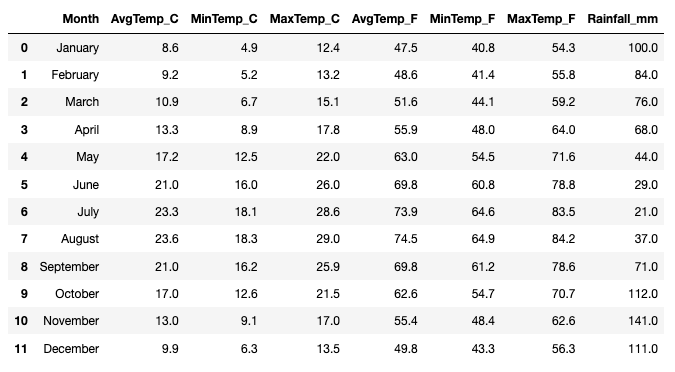
\includegraphics{immagini/df_climate.png}}
		\caption{Climate dataframe for Naples city. }
		\label{fig:df_climate}
	\end{figure}

Let's analyze and visualize these data. 
We can see the trend of temperature in time and by this way also the rainfall in time. 
In figure \ref{fig:np_temp_rain} I reported the trend for averae temperature in degrees centigrade with minimum and maximum variation (left) and a bar plot of the trend for rainfall in mm.

\begin{figure}[!htb]
		\centering
		\scalebox{0.4}[0.45]{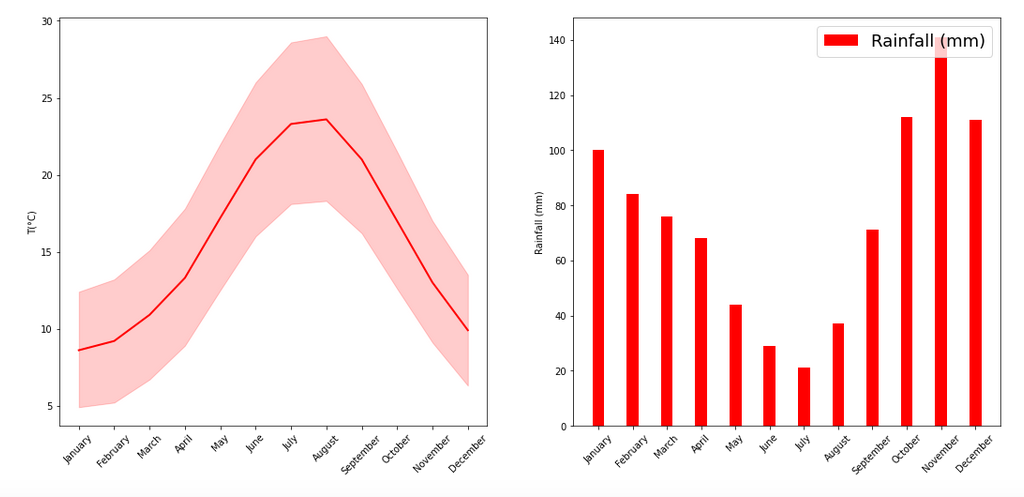
\includegraphics{immagini/np_temp_rain.png}}
		\caption{Trend for average temperature in degrees centigrade (left) and barplot for rainfall in mm (right).}
		\label{fig:np_temp_rain}
	\end{figure}

In order to have a better idea of these data let's do a comparison with another city as New York. In figure \ref{fig:ny_temp_rain} you can see this comparison red for Naples and blu for New York.

\begin{figure}[!htb]
		\centering
		\scalebox{0.4}[0.45]{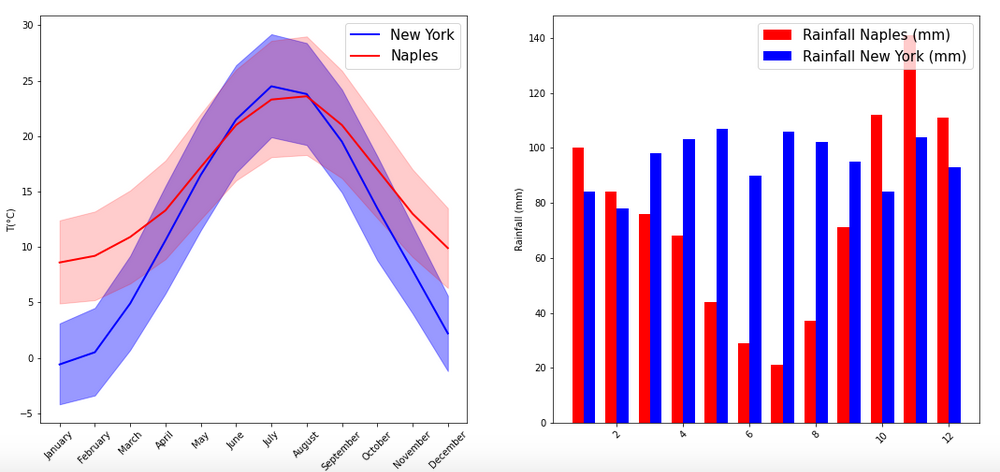
\includegraphics{immagini/ny_temp_rain.png}}
		\caption{Trend for average temperature in degrees centigrade (left) and barplot for rainfall in mm (right).}
		\label{fig:ny_temp_rain}
	\end{figure}

We can see that Naples has generally an higher temperature over $10~ ^{\circ} C$ and a lower rainfall than New York

\begin{thebibliography}{9}
\bibitem{Teleport} 
https://teleport.org/cities/naples/
 
\bibitem{economics}
https://en.wikipedia.org/wiki/Naples

\bibitem{municipalities}
https://it.wikipedia.org/wiki/Municipalit$\%$C3$\%$A0$\_$di$\_$Napoli

\bibitem{opendata}
http://www.comune.napoli.it/flex/cm/pages/ServeBLOB.php/L/IT/IDPagina/26531 

\bibitem{climate}
https://en.climate-data.org/europe/italy/campania/naples-4561/

\bibitem{dataset}
https://github.com/claudio$-$calamita/Coursera$\_$Capstone/tree/master/dataset

\end{thebibliography}
\end{document}